\section{Sudden Insight}

Setup
\begin{itemize}
    \item Figure 3 (c) shows length of paths to water from home. It averages over mice, resulting in a smooth exponential learning curve. As noted in (what's the reference for this again?), averaging over learning curves will always result in a smooth exponential.
    \item Figure 5 (B, C, D) show examples of mice exhibiting discontinuous learning, demonstrated by an abrupt change in gradient of the cumulative number of direct paths to water over time.
    \item This sudden insight behaviour was noted in 5 of the 10 mice
    \item We study each mouse individually to determine if they exhibit discontinuous learning. We also attempt to detect the point of sudden insight using two methods.
    \item Firstly, we analyse the numer of steps each mouse takes to arrive at the water port from home. These are shown as a blue scatter in <insert figure>. We assume that the pre and post insight distributions of these path lengths are statistically different. We use a Bayesian Change Point etection algorithm to determine the optimal location of separation under the assumption that path lengths before and after the separation are drawn from two distinct Poisson distributions.
    \item Insert equation
    \item These are shown in red on <insert figure>. The pre-post distributions are shown alongside the main plot and scatter points shown in light blue for pre insight and dark blue for post insight.
    \item We include a Mann-Whitney U test to determine if the pre and post insight distributions are statistically different.
    \item Insert equations
    \item Secondly, we analyse the number of cumulative direct paths to water, where a direct path is one which passes between home and the water port along the single optimal 6 node path. We detect an abrupt change in rate of this curve using the <name of algorithm>, in which we determine the point of maximum distance from a line connecting the first and last points of the cummulative curve.
    \item Insert equation
    \item These are shown in green on <insert figure>, which attempts to detect.
    \item In addition to showing these detailed plots for two mice exhibiting both continuous and discontinuous learning, we also include a summary plot for all mice in <insert figure>
    \item This plot shows the detected changepoints, as well as the occurance of both direct paths and water port rewards.
\end{itemize}

Observations
\begin{itemize}
    \item Prior to their first direct path to water, mice tend to exhibit longer initial exploration paths, taking longer to reach the water port. In some cases, following the first direct path to water, these paths will occur with consistent high frequency for the remainder of the experiment. 
    \item Both the time of first direct path and number of occurences before settling into a consistent frequency vary across mice, shown in <figure C> with a green '+'.
    \item We note that many rewards may be accumulated prior to the first direct path, though this is not necessarily corelated with sudden insight, and in many cases we see a consistent linear increase in cumulative rewards.
    \item We also note that exploratory behaviour is still present following sudden insight, though paths to water tend to drop following the insight.
    \item We also note that both the elbow and change point detectors are well correlated in cases where they occur early, however they are less correlated in cases where they occur later.
    \item Though direct paths acts as an indicator of discontinuous learning, we also observe a gradual decrease in path length of non-direct paths, which results in decorrelation of the two detectors.
    \item This may indicate a distinction between "learning where the water is" and "learning how to get to the water from home". If present, would suggest learning of both an internal maze representation and a set of heuristics for optimal water port exploitation.
    \item 
\end{itemize}


\begin{figure}
    \centering
    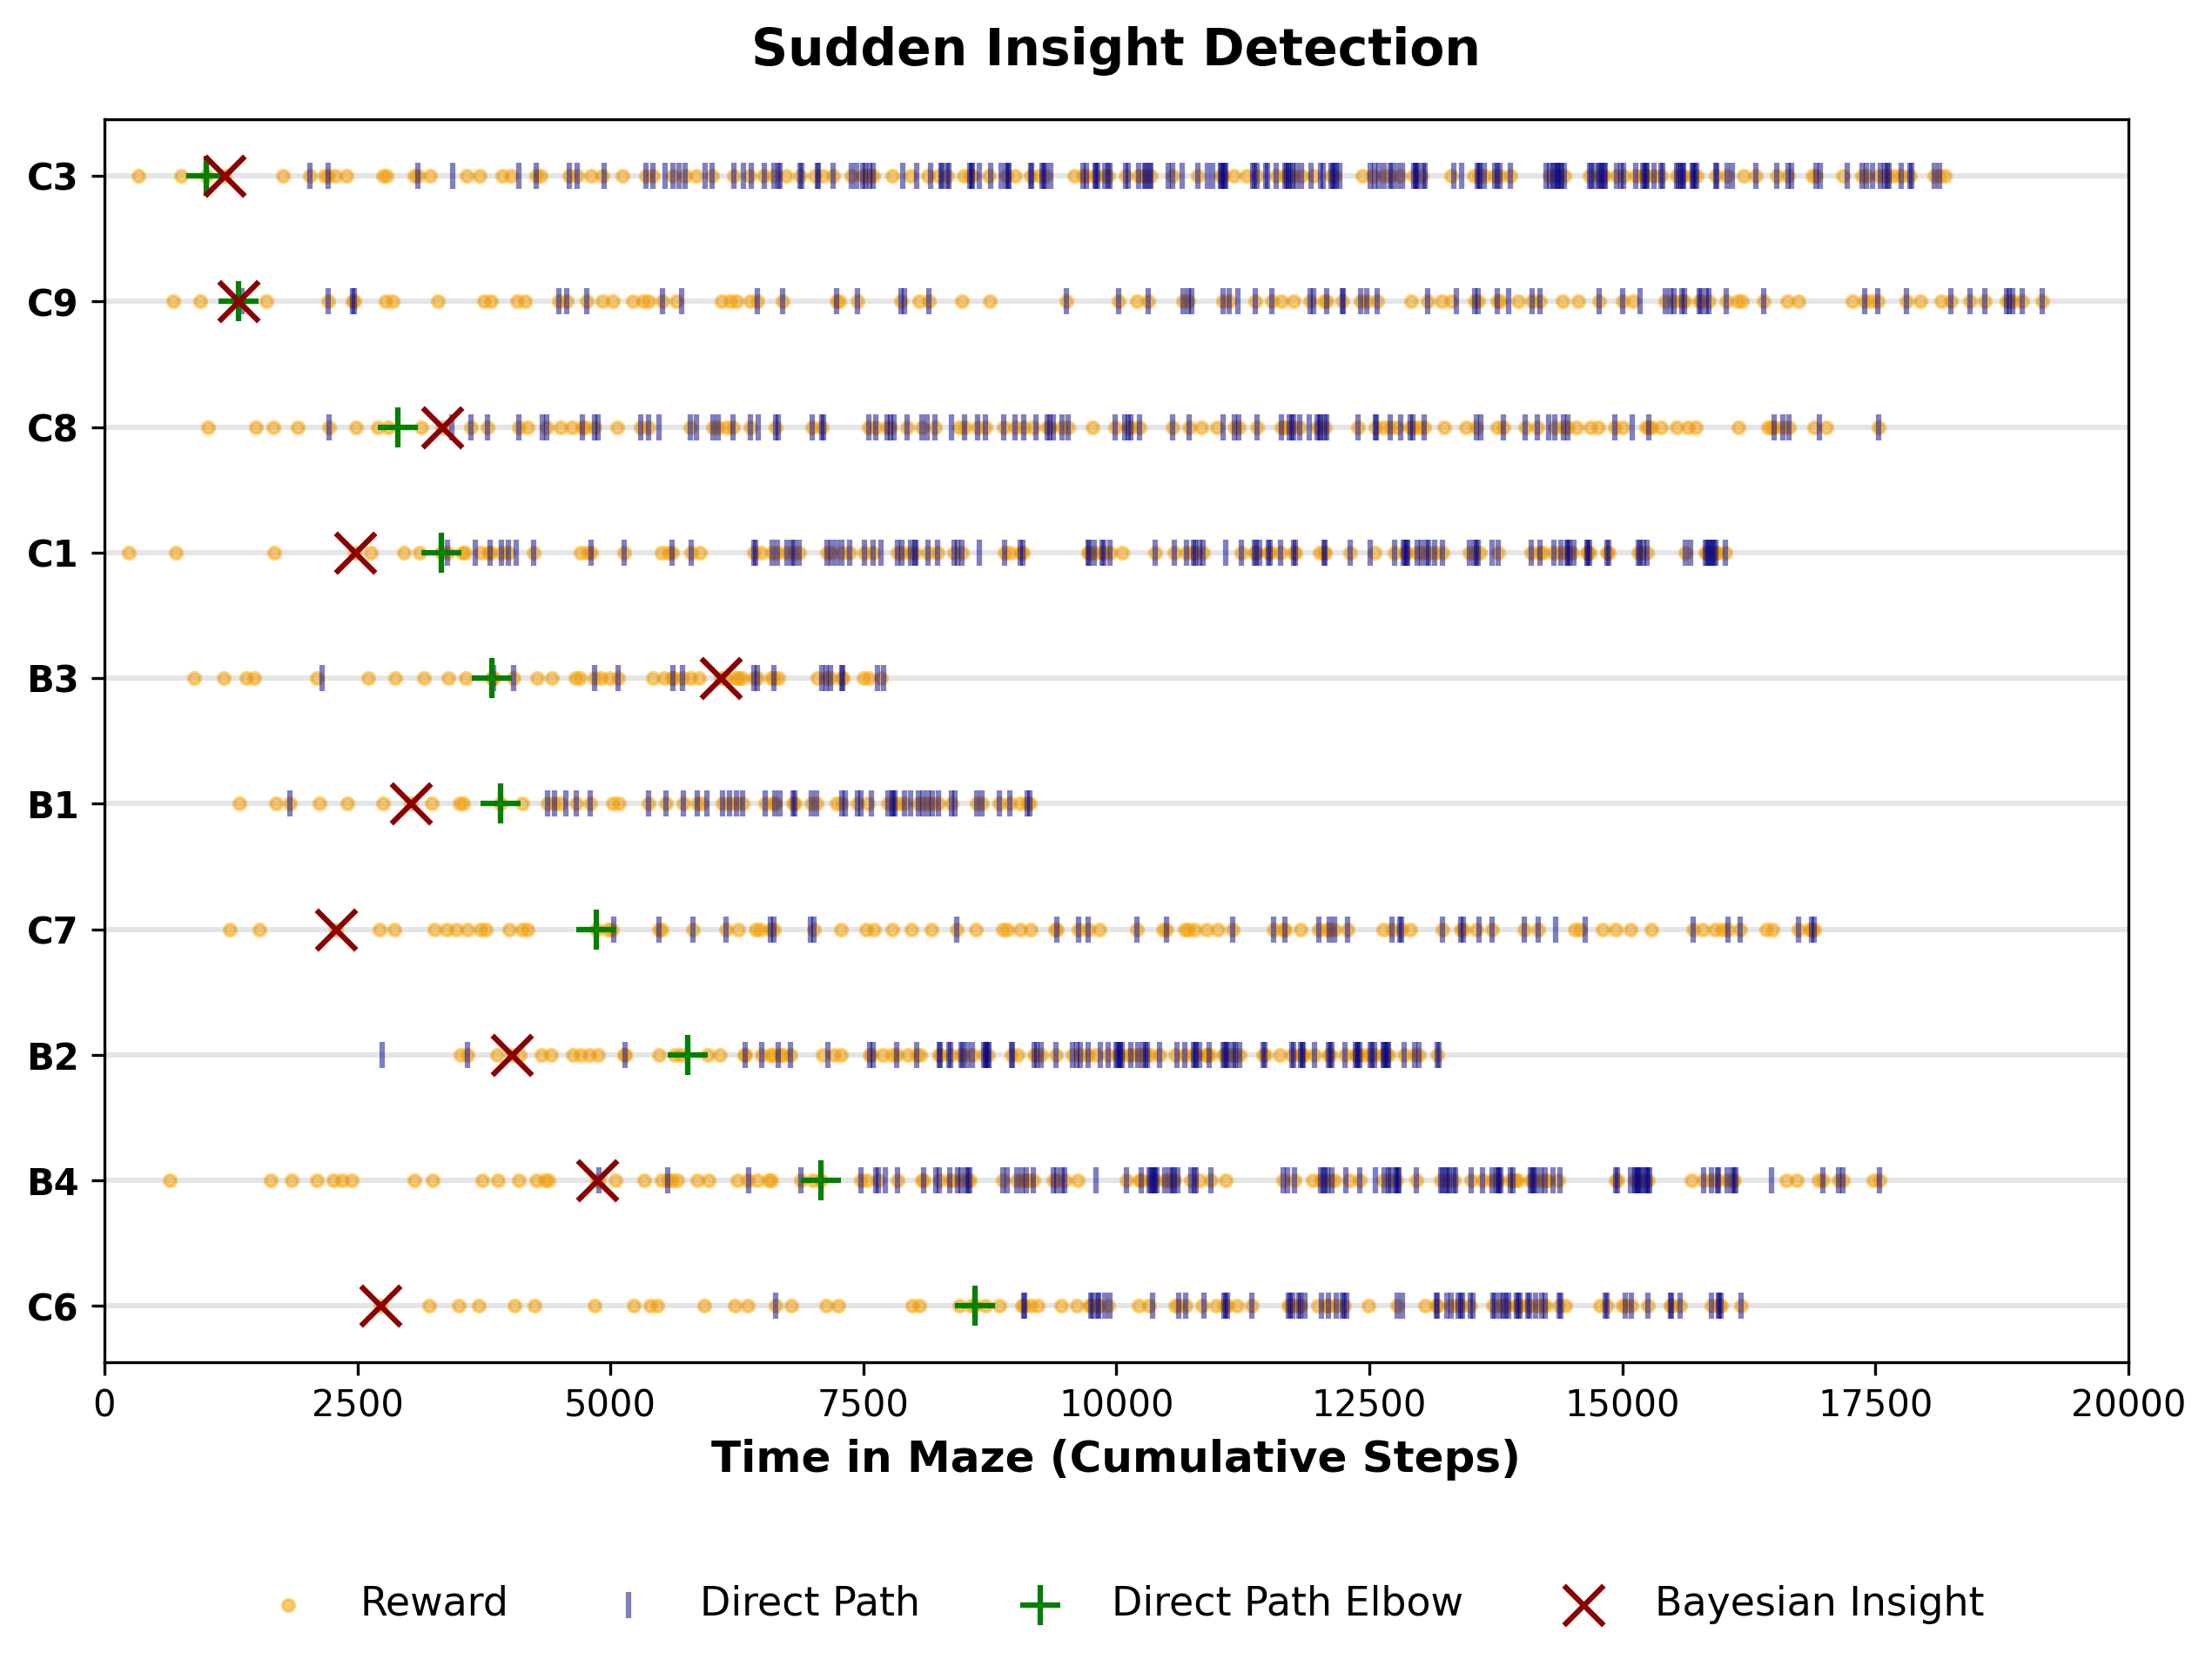
\includegraphics[width=\singlefigure]{figures/sudden_insight_all.png}
    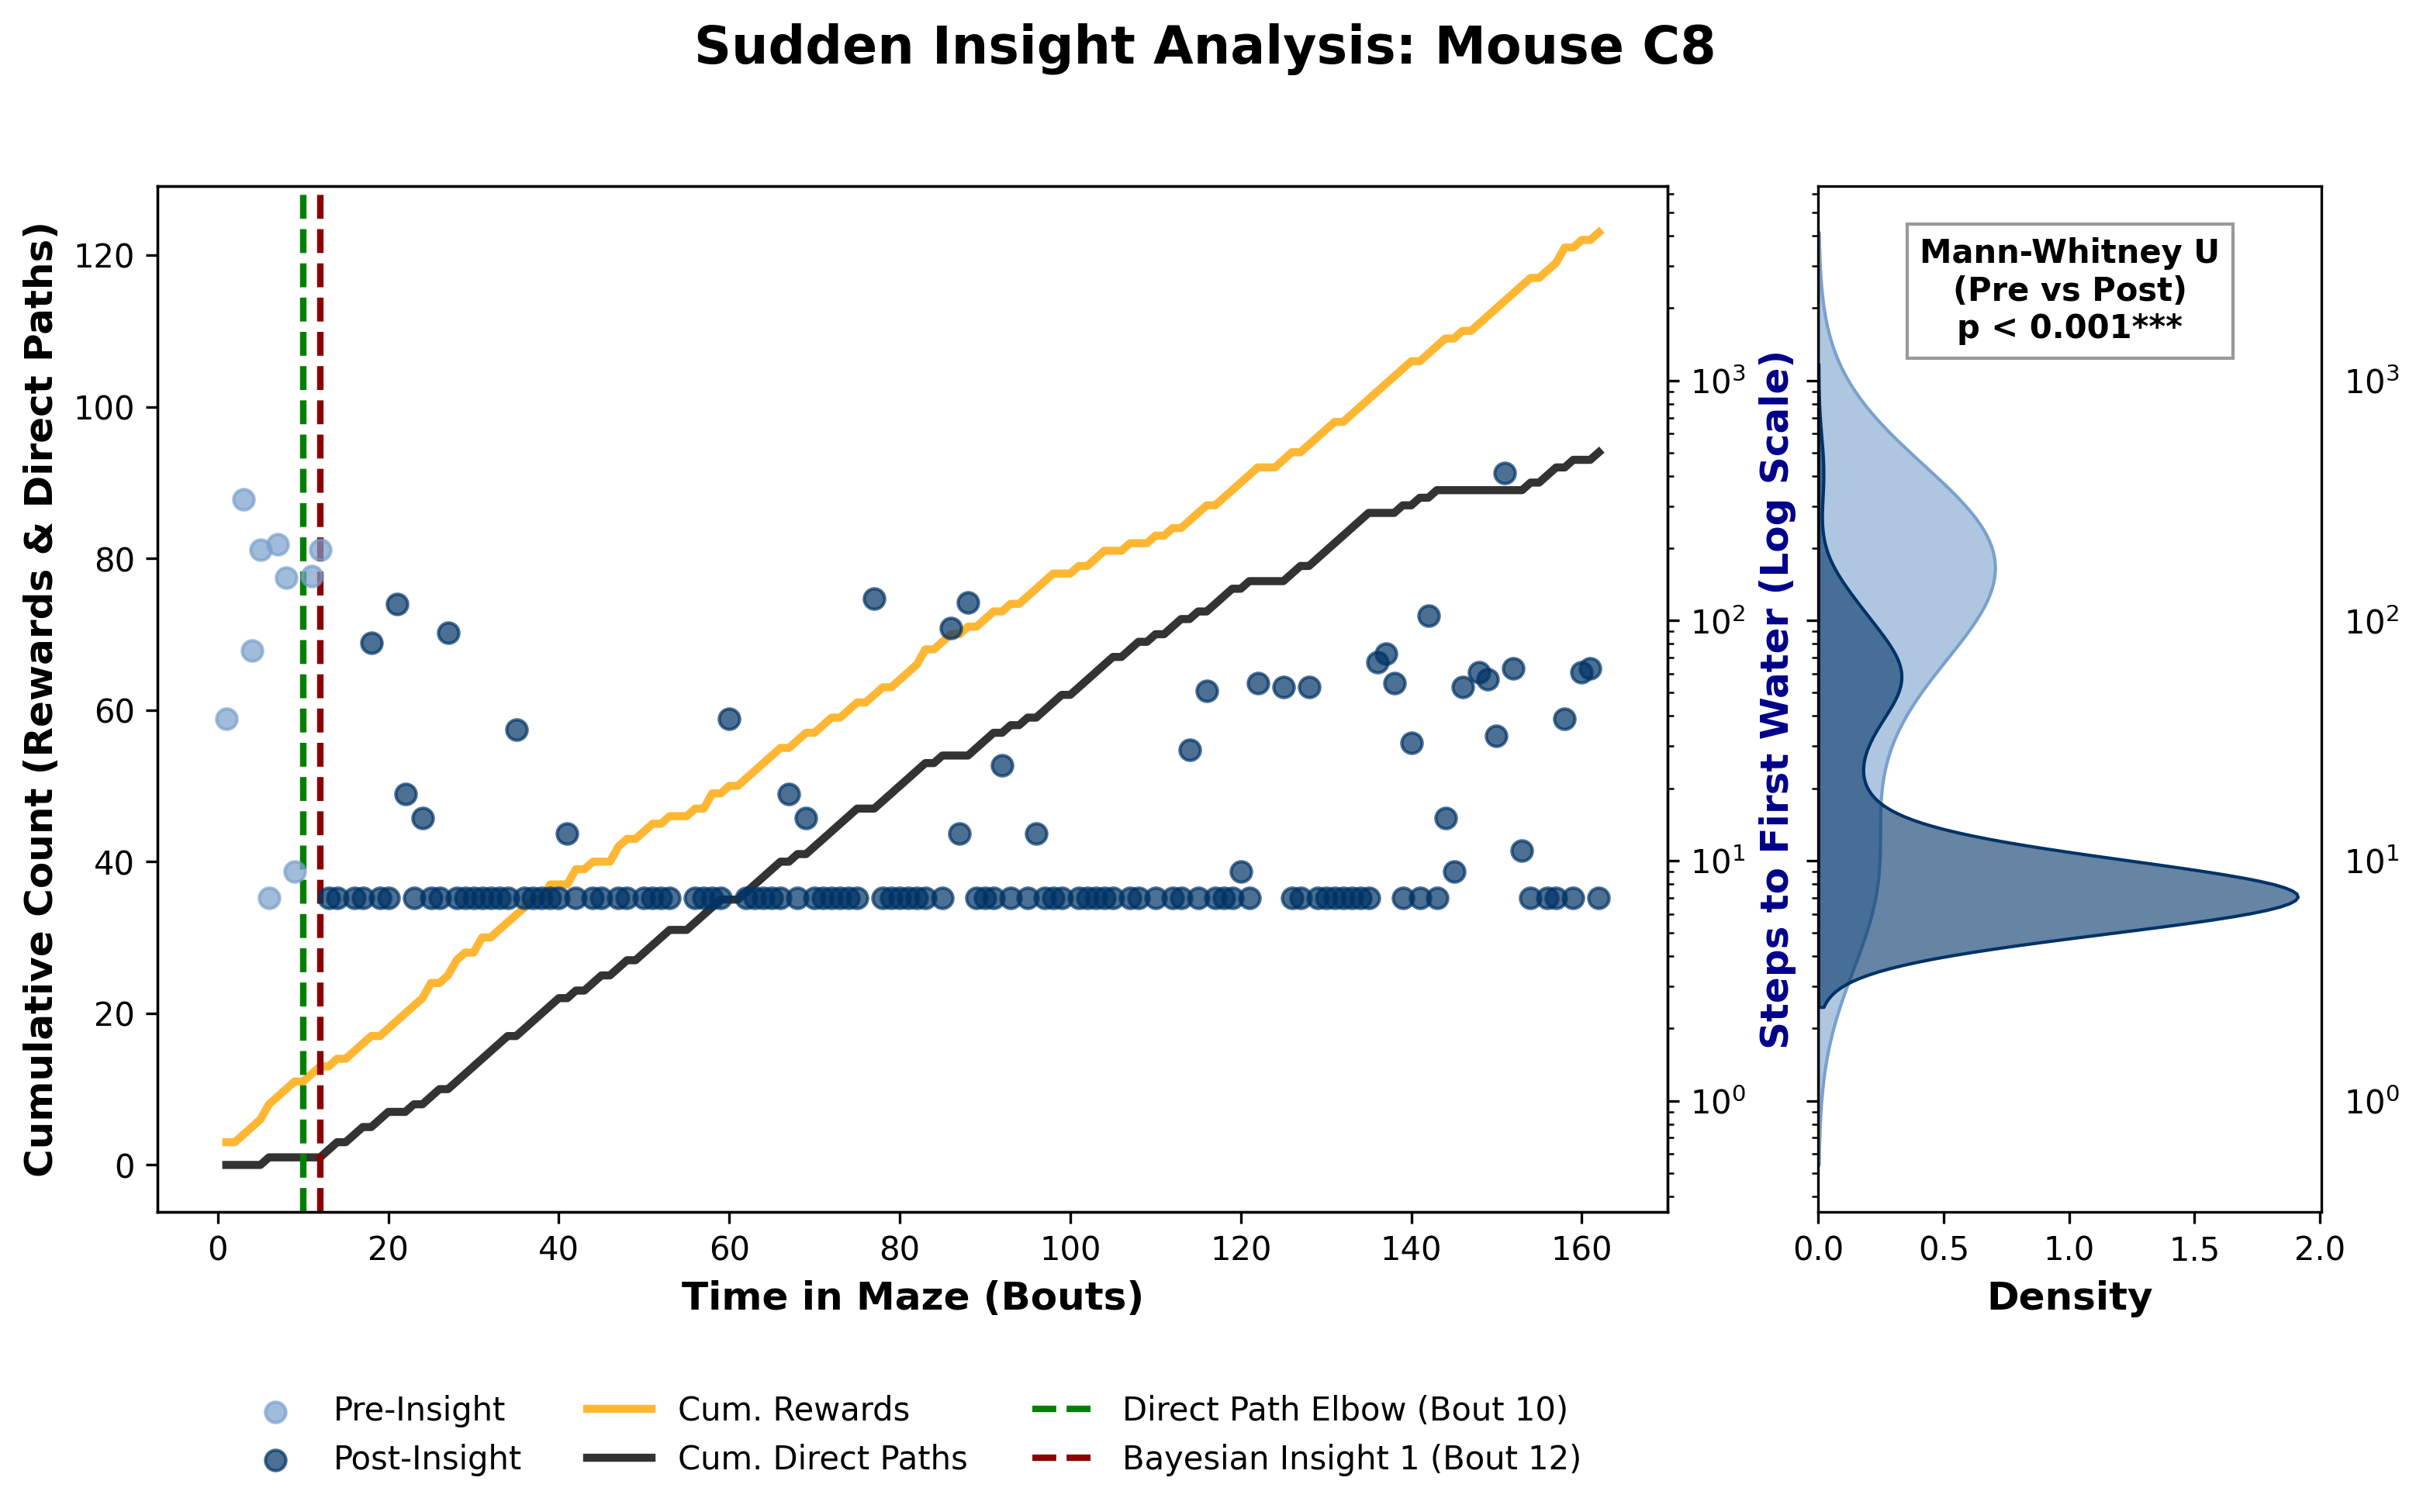
\includegraphics[width=\singlefigure]{figures/sudden_insight_C8.png}
    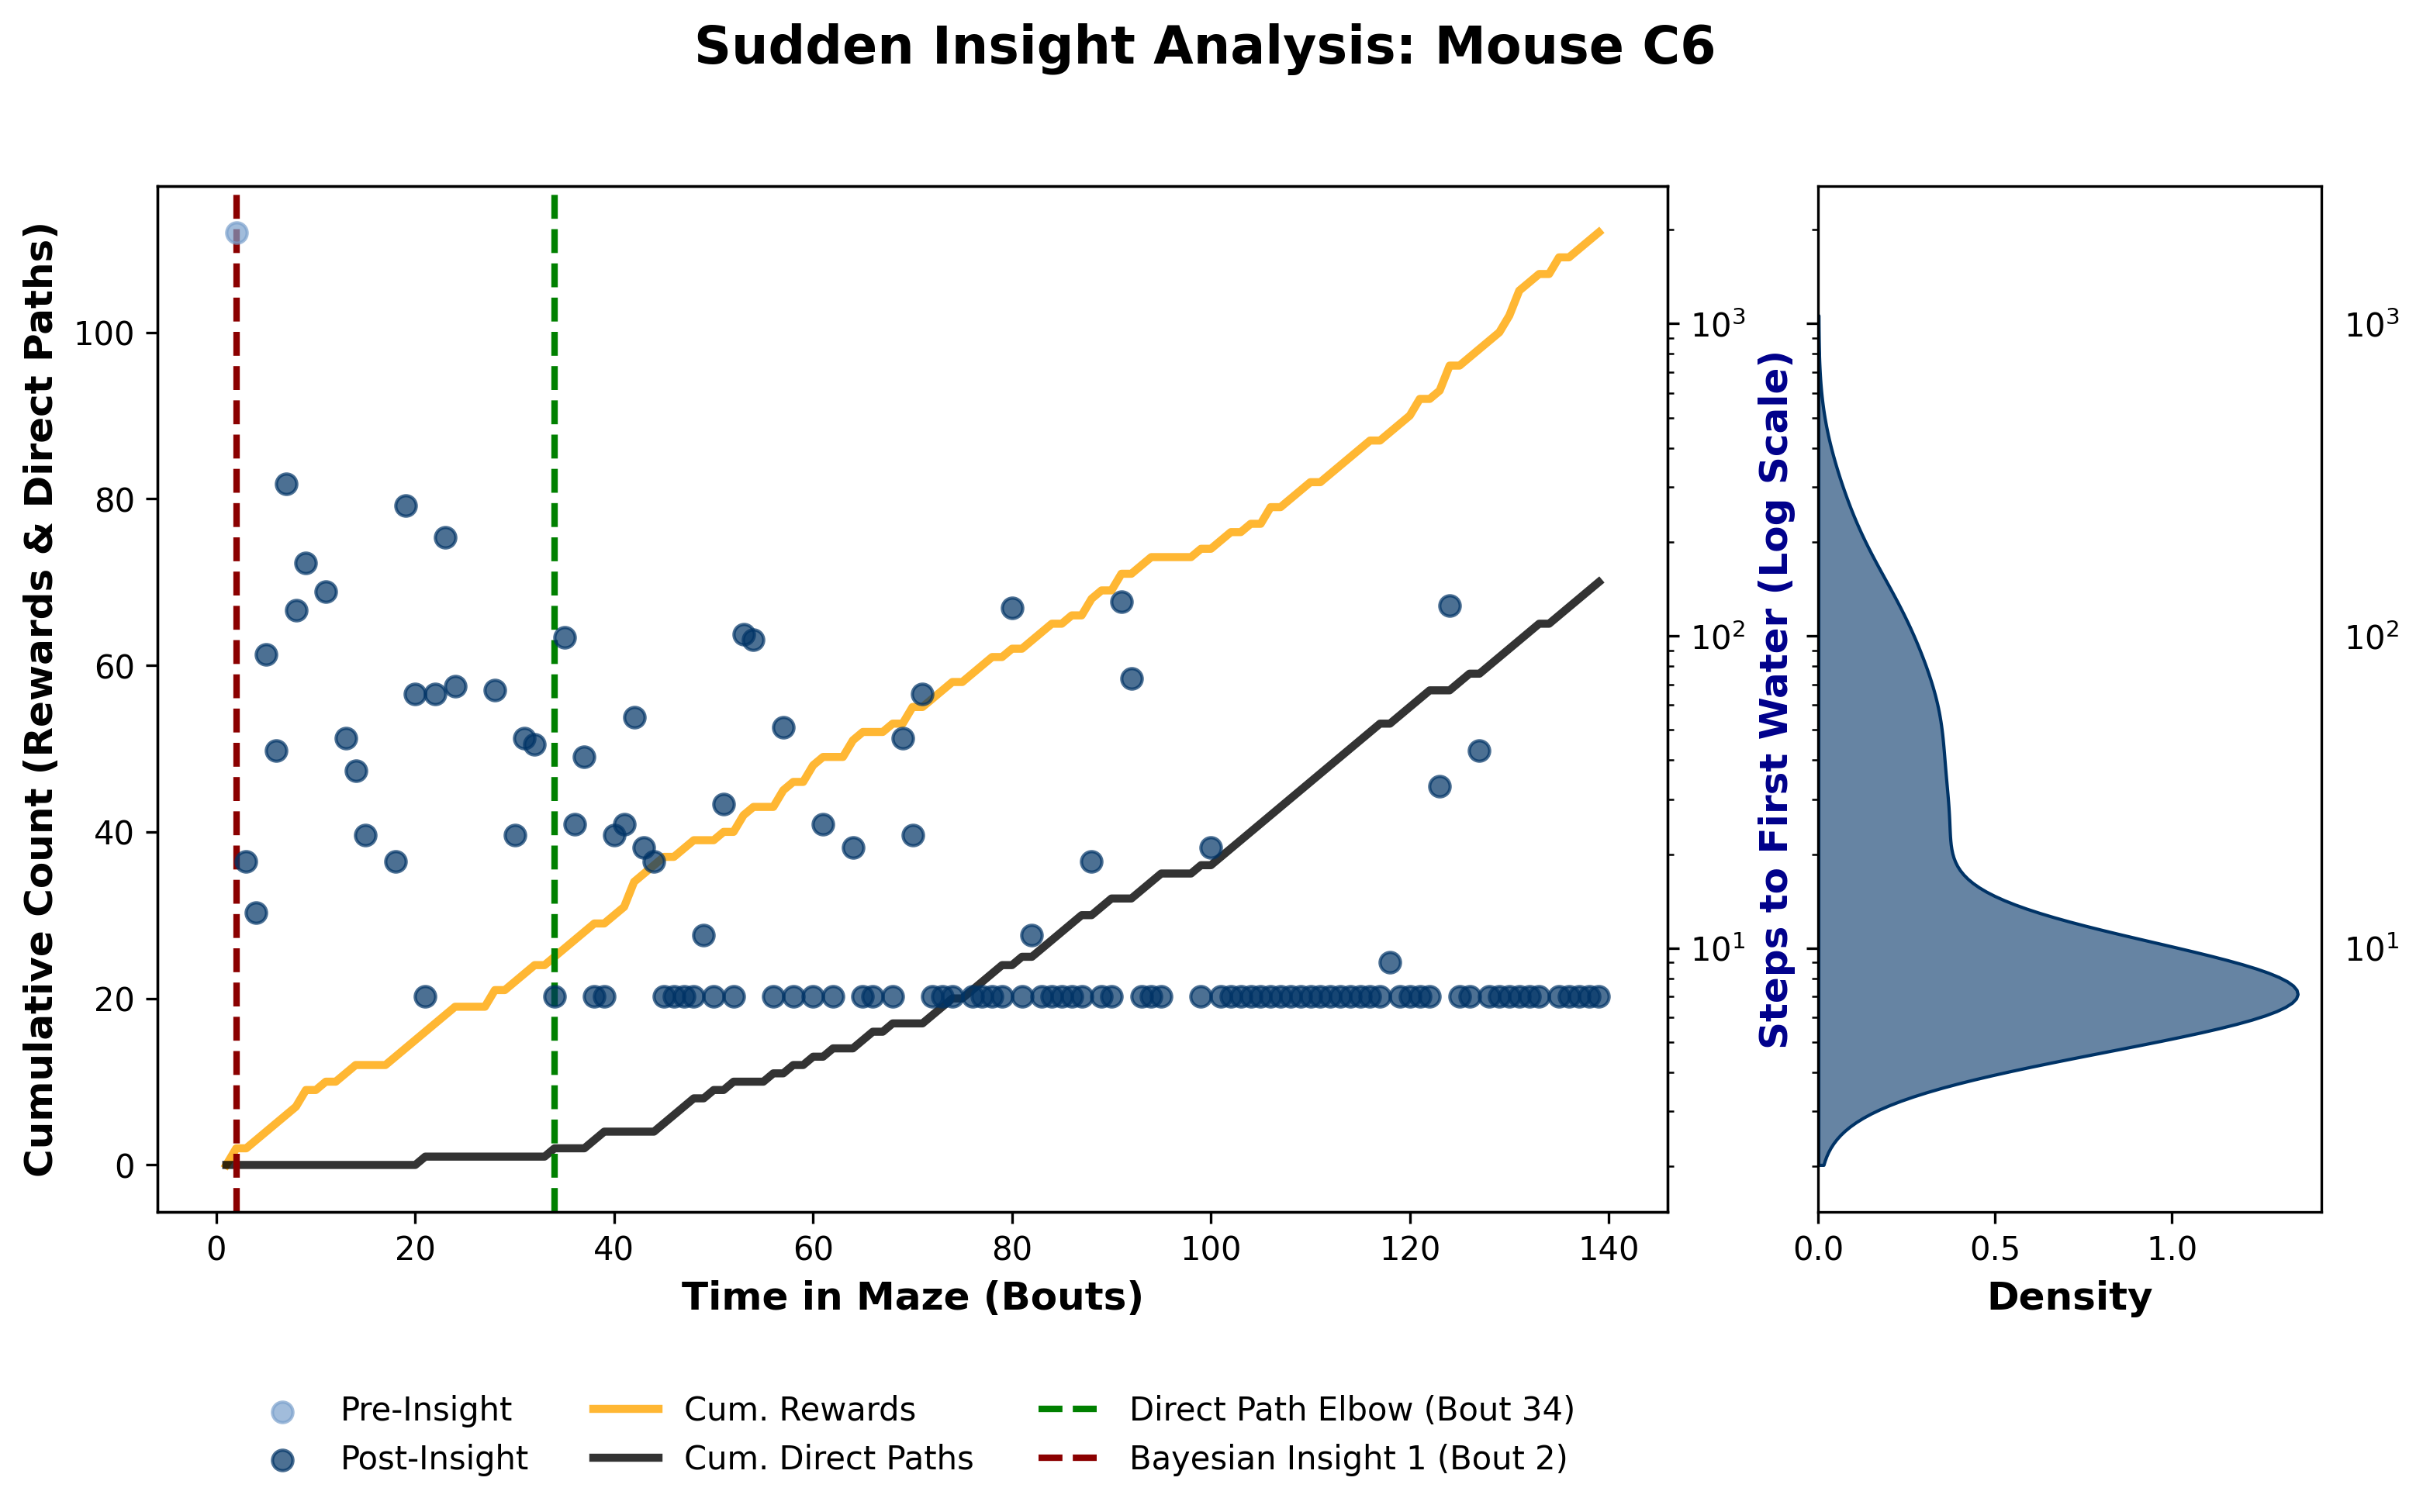
\includegraphics[width=\singlefigure]{figures/sudden_insight_C6.png}
    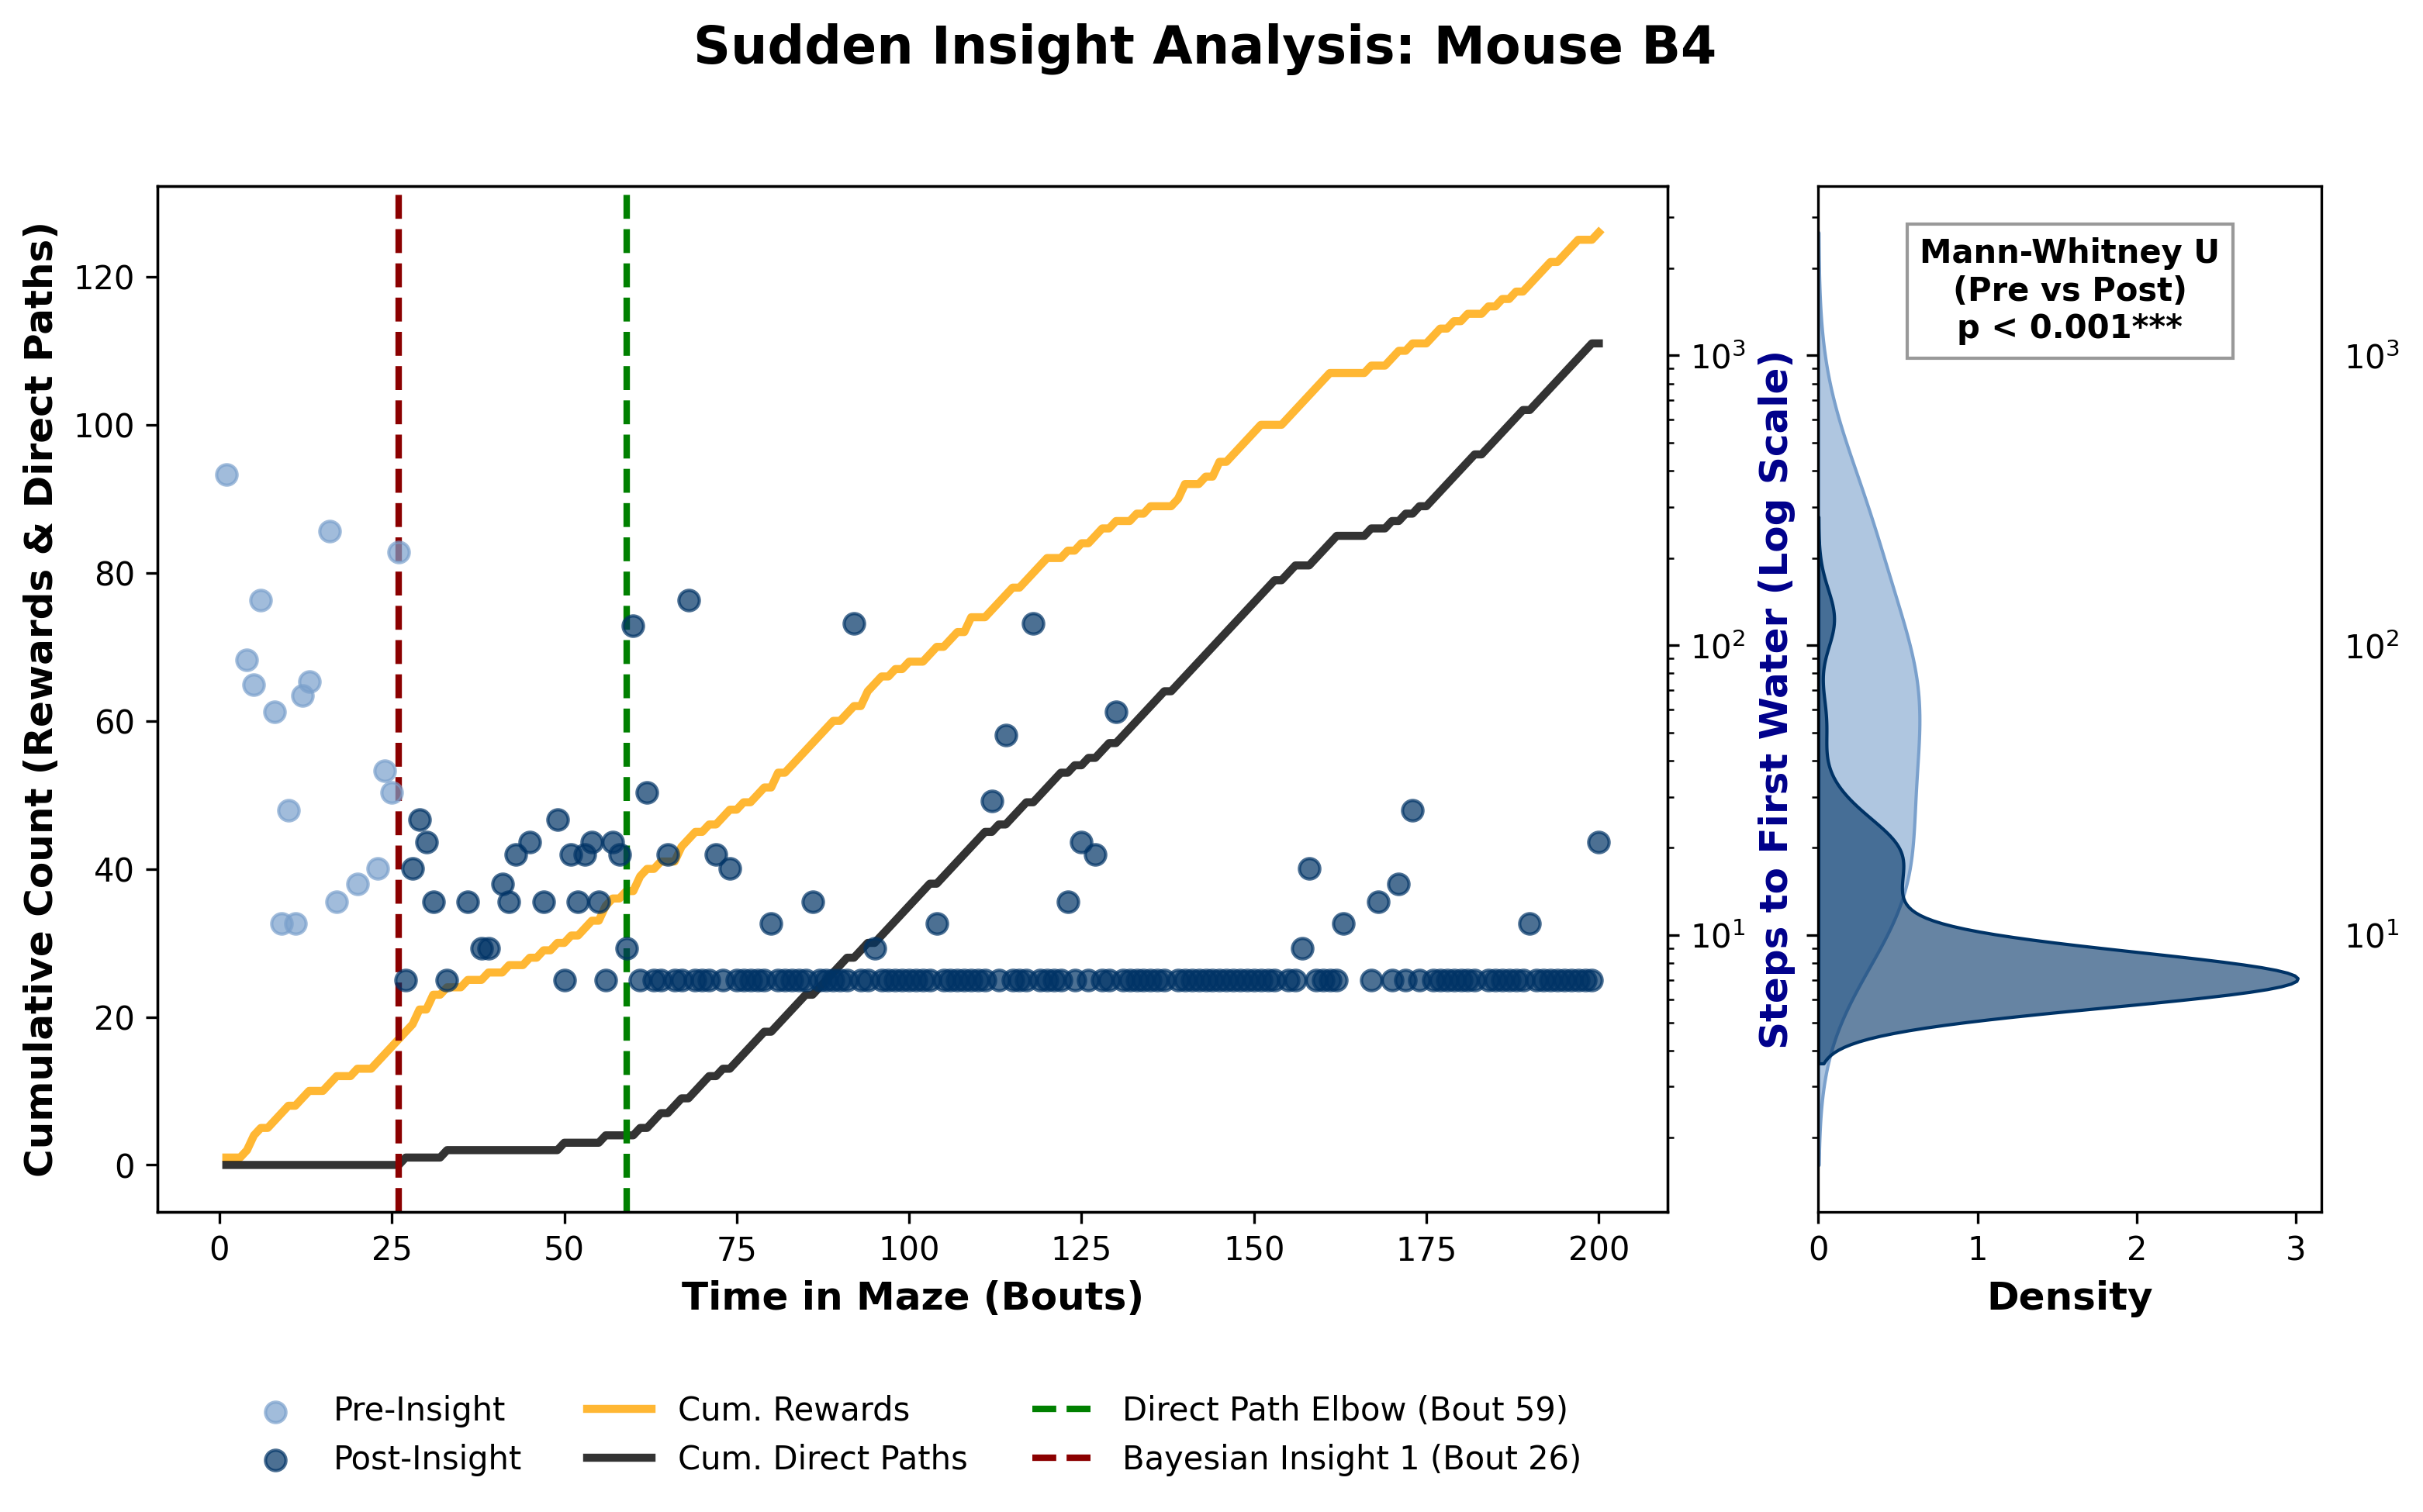
\includegraphics[width=\singlefigure]{figures/sudden_insight_B4.png}
\end{figure}